\section{Results}\label{sec:results}

\subsection{M\"obius Results}\label{sec:mobiusresults}

One surprising result of this simulation involved the \texttt{num\_replicas} parameter, which controlled the number of copies of the operating system image saved on an individual device.  When we first ran this simulation, we believed that our model was incorrect because the system reliability was completely unaffected by the \texttt{num\_replicas} parameter.  In order to further debug the system, we added additional places to the model to keep track of the number of SEU and SEFI events that were recorded in the system.  To our surprise, M\"obius reported that an average of 0.0 SEU events (with 95\% confidence interval width 0.0) occured over 1000 simulation runs; as M\"obius reports small numbers that it can detect, this average likely indicates that no SEU occured during each of the 1000 simulations.  In retrospect, this conclusion is reasonable; the SEU error rate is on the order of $10^{-7}$ events per day, which corresponds to an average time before failure of over 27,000 years.  In addition, an SEU only corrupts a kernel if it modifies any of the data in that kernel.  We assumed that each kernel took up 10MB of space and that errors were uniformly distributed across the 512MB flash chip.  As a result, any SEU that occurred had a $\frac{10\cdot\textrm{number of kernels}}{512}$ chance of actually corrupting a kernel.  These two factors combined indicated that the probability of an SEU affecting a kernel on the given Micron flash memory was essentially zero.

As the probability of an SEU event in this model affecting a kernel was essentially zero, we recognized that controlling SEFI events was the key toward maintaining reliable operation.  In order to accomplish this goal, we expanded our model to include $n$ independent devices, each containing $m$ copies of the kernel.  Each device has its own controller hardware and fails independently, so the system is able to handle $n-1$ SEFIs without failing.  We also focused on testing the periodic reboot parameter discussed in Section \ref{sec:buildingmodel}.

The results of this simulation are shown in Figure \ref{fig:reliability} and Table \ref{tab:reliability}.  The 95\% confidence interval width is plotted for each point in Figure \ref{fig:reliability} and is also included in Table \ref{tab:reliability}

\begin{figure}[width = 0.5\textwidth]
\centering
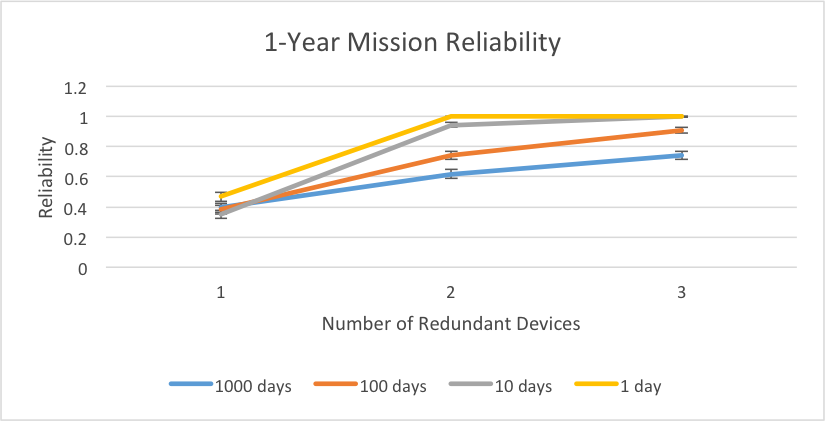
\includegraphics[scale=0.6]{reliability}
\caption{1-year mission reliability for our model}\label{fig:reliability}
\end{figure}

\begin{table}[width = 0.5\textwidth]
\centering
\begin{tabular}{|c|c|c|c|c|}
\hline
& \multicolumn{4}{|c|}{\bf Flash Reboot Interval (days)}\\
\hline
{\bf \# Dev} & 1000 & 100 & 10 & 1\\
\hline
1 & 0.395 $\pm$ 0.030 & 0.383 $\pm$ 0.030 & 0.351 $\pm$ 0.030 & 0.468 $\pm$ 0.031 \\
2 & 0.618 $\pm$ 0.030 & 0.741 $\pm$ 0.028 & 0.944 $\pm$ 0.014 & 0.998 $\pm$ 0.001 \\
3 & 0.740 $\pm$ 0.027 & 0.908 $\pm$ 0.018 & 0.998 $\pm$ 0.003 & 1.000 $\pm$ 0.000 \\
\hline
\end{tabular}
\caption{1-year mission reliability for our model}\label{tab:reliability}
\end{table}

As the graphs indicate, the default reliability of the IlliniSAT system is fairly low; there is approximately a 40\% chance that the satellite will survive a year under this model.  However, the introduction of another device improves reliability slightly.  If at least two devices are available, periodically power-cycling the Flash memory provides an additional, significant reliability improvement.  If the Flash is power cycled daily, we are able to achieve an estimated reliability of 99.8\%, a significant improvement over our initial condition.
\subsection{Fault Injection Tool}
